\chapter{Vergleich entwickelter Rekonstruktions Algorithmus mit bereits vorhandenen (Matlab)}
\label{sec:rectification}

(ÜBERSCHRIFT ÄNDERN!)\\

\textcolor{red}{(Der entwickelte Szenenrekonstruktionsalgorithmus wurde so entwickelt, dass eine Rektifizierung der Bilder, wie sie in vielen Programmen verwendet wird, nicht notwendig wird. Der Grund dafür ist, dass ein Algorithmus entsteht, welche auch mit Bildern unterschiedlicher Kameraauflösungen eine erfolgreiche Rekonstruktion vollbringt) Ausbauen, verbessern, genauer erklären wie warum, was ist mit rektifizierung gemeint, irgendwo mss noch die vorgeschichte dazu rein... Matlab verwendet verfahren über fundamentalmatrix und rektifizierung, problem: kommt nicht mit anderen Kameraauflösungen zurecht. Zwei lösungen: einmal rekonstruktion über essentielle matrix oder neuer rektifizierungsalgorithmus. Ansatz im anderen Kapitel....Hier soll es eher darum gehen den eigenem Ansatz mit dem aus Matlab zu vergleichen und auf das Prblem der Rektifizierung in Mtlab eingehen. Den hierigen Rektifizierungsansatz mit dem aus maltlab vergleichen.Problem der unterschiedlich großen Bilder ansprechen. Mein Ansatz rekonsturiert ohne dei ausgabebilder zu "kennen" und zu verändern, bbei rektifizierung wird mit den feriten Bildern gearbeitet, was bei unterschiedlichen Auflösungen zu starken verzerrungen kommen kann bei der Rektifizierung.}\\







Arbeitsprozess Matlab eifügen 

\begin{minipage}{\linewidth}
	\centering
	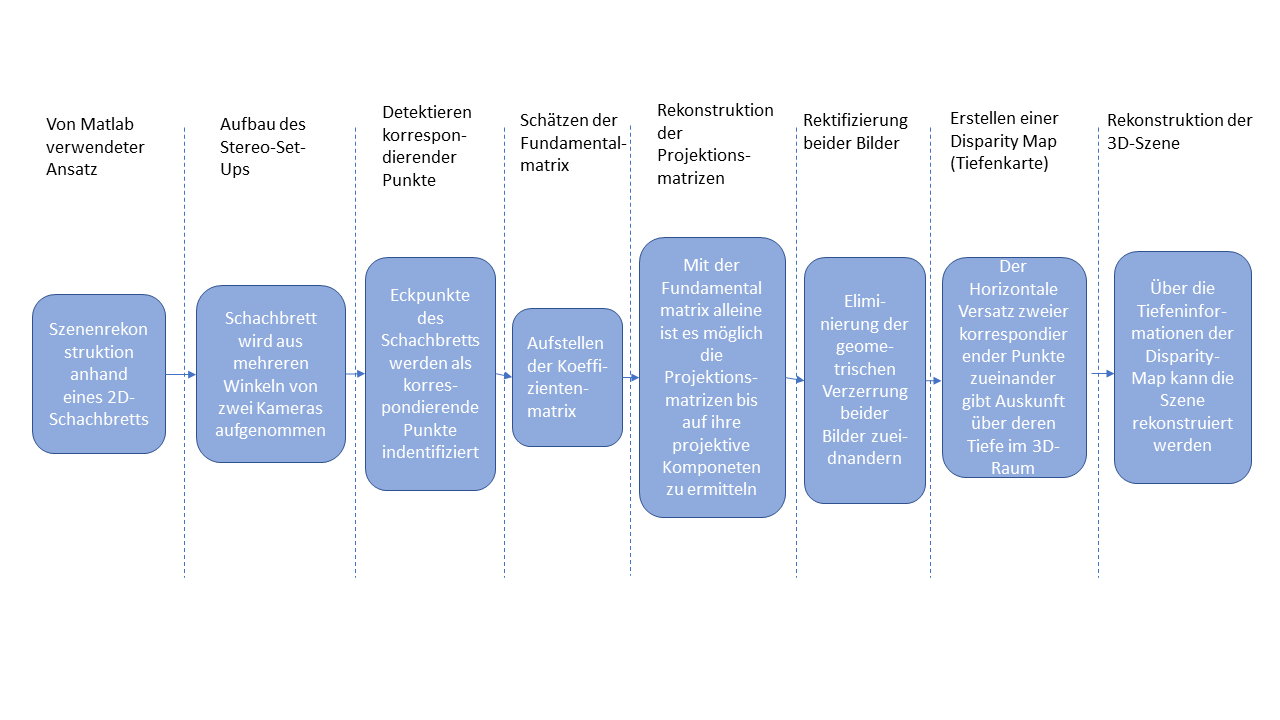
\includegraphics[width=0.8\linewidth]{images/ArbeitsProzessRealunkalibriert.png}
	\captionof{figure}{(Überarbeiten sie Abb \ref{fig:ArbeitsProzessVirtuell})Durch Ungenauigkeiten in der korrespondierenden Punkte, verfehlen sich die Linien und es kommt zu keinem Schnittpunkt} 
\end{minipage}\\ 



%
%Im Minimalbeispiel ist die Triangulierung und Rekonstruktion der 3D-Weltpunkte ohne Kommunikationen durchführbar. Das liegt daran, dass mit reinen Werten gerechnet wird und Fehler wie Beispielsweise Bildrauschen nicht vorkommen. Im Minimalbeispiel kann davon ausgegangen werden ,dass die Linien zweier korrespondierender Punkte sich, welche durch die jeweilien Kamerazentren und Bildpunkte gehen, sich ziemlich sicher in einem Punkt treffen werden. In einem Beispiel mit realen Daten ist es nicht unwahrscheinlich, dass die herausgefilterten korrespondierenden Punkte, nicht zu hundert Prozent stimmen. Es kommt immer zu kleineren Abweichungen, was dazu führen kann, dass wenn die Linien der korrespondierenden Punkte im Realbild sich nicht treffen. Ein Grund dafür ist, dass sie nicht hundertprozentig auf der selben Höhe im Bild liegen und die Linien sich somit verfehlen\\
%
%
%
%\begin{minipage}{\linewidth}
%	\centering
%	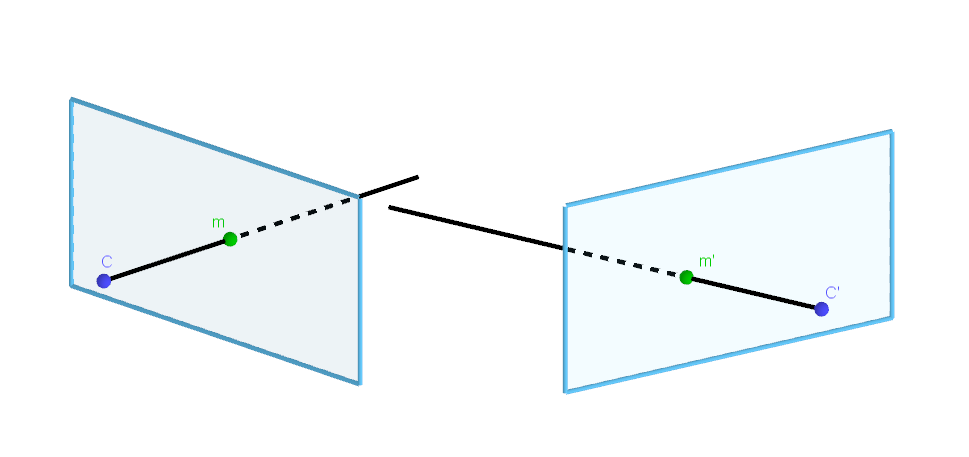
\includegraphics[width=0.8\linewidth]{images/problemTriangulation.png}
%	\captionof{figure}{Durch Ungenauigkeiten in der korrespondierenden Punkte, verfehlen sich die Linien und es kommt zu keinem Schnittpunkt} 
%\end{minipage}\\ 
%
%
%
%
% Im Realbeispiel dieser Arbeit wird das Auftreten solcher Fehler durch das sogenannte \textit{Sampson-Approximation} - Verfahren behoben, welches bei kalibrierten Fällen zum einsatz kommt\cite{HZ}. Mehr zu diesem Verfahren wird im Kapitel \nameref{sec:sampson} aufgeführt. Das ist eine Möglichkeit um eine Szenerekonstruktion trotz Fehlerhafter korrespondierender Punkte zu ermöglichen. 
Ein weiteres weit verbreitetes Verfahren, ist cor der Szenenrekonstruierung durch Triangulierung eine Rektifizierung beider Bilder vorzunehmen\cite{MatlabRec,ZZ,Javier,Fusiello}. Da bestimmte Formen der Rektifizierung keine vorherige Kalibrierung der Kameras benötigen, wird diese Methode in den meisten gängigen Echtzeit-Szenenrekonstruktionen eingesetzt. \cite{Fusiello,Javier,R.H.}.
Rektifizierte Bilder müssen zwei Eigenschaften erfüllen. Zum einen müssen alle Epipolargeraden parallel zur x-Koordinatenachse verlaufen und zweitens müssen alle korrespondierenden Punkte die selben y-Koordinaten besitzen\cite{ZZ}. Mit Hilfe dieser Eigenschaften ist es somit möglich die enstandenen korresponierenden Epipolarlinien als horizontale Scanlinien zu benutzen\cite{Javier,ZZ}. Mit hilfe dieser Scanlinien und den darauf sich befindenden korrespondierenden Punkte ist es zum Beispiel Möglich eine Tiefenkarte des Bildes zu berechnen allein durch die Differenz der horizontalen Lage der korrespondierenden Punkte\cite{Javier,ZZ}. \\
 
 
 \begin{minipage}{\linewidth}
 	\centering
 	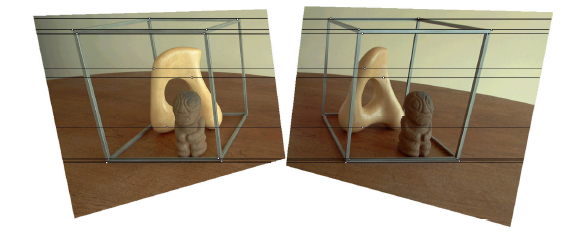
\includegraphics[width=.8\linewidth]{images/rectifiziertesBildAusZZ.png}
 	\captionof{figure}{Beipiel eines rektifizierten Bildes. Quelle: \cite{ZZ}} 
 \end{minipage}\\ \\

 \begin{minipage}{\linewidth}
	\centering
	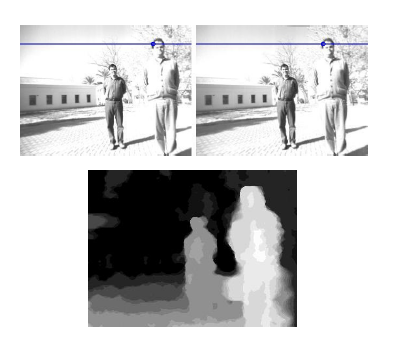
\includegraphics[width=.8\linewidth]{images/Disparity.png}
	\captionof{figure}{Beispiel einer einfachen Tiefenkarte eines Stereobildpaares nach der Rektifizierung. Quelle: \cite{Javier}} 
\end{minipage}\\ \\
 
Die Rektifizierung, allem voraus vor allem die Optimierung des Rektifizierungvorgangs, von Stereo- oder auch mulitplen- Kamerasystemen, wird heutzutage von vielen Entwicklergruppen der Computer Vision untersucht(Der satz ist mist!). Es gibt mittlerweile viele Ansätze, jedoch funktionieren nicht alle bei den selben Fällen. So setzten zum Beispiel manche Rektifizerungsalgorithmen voraus, dass die Bilder von Kameras mit selber Auflösung aufgenommen wurden. Ein Beispiel ist die Rektifizierung welche in \textit{Matlab} verwendet wird \cite{MatlabRec}. Die Rektifizierung wurde anhand einer Methode implementiert, welcher sich ähnlich verhält wie in \cite{FusielloSite} beschrieben. Die Grundidee hier hinter ist, dass die Kameramatrizen von zwei Kameras so aufgebaut sind dass die intrinsischen Parameter die selben sind, sie sich aber in ihren Rotationen und Translationen voneinander unterscheiden. Die extrinsischen Kameraparameter werden dann dementsprechend so manipuliert, dass die Bildebenen Achsenparallel zueinander stehen\cite{FusielloSite,Fusiello}. Um horizontale Epipolarlinien zu erhalten muss gleichzeitig die Basislinie zwischen den zwei Kamerazentren parallel zur neuen x-Achse beider Kameras sein. Zudem soll, um eine angemessene Rektifizierung zu gewährleisten, müssen konjugierende Punkte die selbe vertikale Koordinate haben. Dies wird hier durch die die Bedingung gewährleistet, dass beide Kameras die selben intrinsischen Parameter haben\cite{FusielloSite}. Eine Frage welche mit unter in dieser Arbeit beantwortet werden sollte, war, ob es möglich ist, ohne deutlich größeren Aufwand eine Kamerakalibrierung und Szenerekonstruktion mit Kameras unterschiedlicher Auflösung zu gewährleisten. Im Kapitel \nameref{sec:epipolar}, in welchem ausführlich die Epipolargeometrie vorgestellt wurde, wurde bereits bezug auf die unterschiedlichen Auflösungen genommen. Prinzipiell spielen unterschiedliche intrinsische Kameraparameter keine Rolle, wenn es um die Rekonstruktion der Kameraposen geht, da die Fundamental Matrix und die essentielle Matrix die Information über die intrinsischen und extrinsischen Kameraparameter besitzen und es klar gestellt wurde, dass die Bildkoordinatensysteme der Kameras nicht identisch sein müssen. \cite{Elements}. \\



In dieser Arbeit wurde ein Rektifizierungsalgorithmus nach \textit{Zhang}\cite{ZZ} implementiert, welcher sich die Fundamentalmatrix zu nutzen macht. \textit{Loop} und \textit{Zhang} zerlegen jede Kollinearität in eine Ähnlichkeitstransformation, eine Schertransformation und eine projektive Transformation. Die projektive Komponenten wird dabei in einem nichtlinearen Optimierungsprozess so affin wie möglich gemacht.\cite{Fusiello,ZZ,phdextrinsicPara}. Im folgenden wird zunächst der genaue Vorgang des implementierten Algorithmus genauer erklärt und 
\textcolor{red}{des Weiteren werden zwei Beispiele vorgestellt, welche die Bilder des Minimalbeispiels einmal mit gleichen intrinsischen Parametern und einmal mit unterschiedlichen intrinsischen Parametern der Kamera aufzeigt. Es wird sich Herausstellen, dass beide Beispiele eine gelungene Rektifizierung der Bilder aufweisen.(Nochmal genau nachprüfen ob das geht!!!)}. \\


Während sich einige Rektifizierungsverfahren im 3D-Raum abspielen, wird beim Verfahren nach \textit{Zhang}, hauptsächlich im 2D-Raum gearbeitet. Des Weiteren wird vorausgesetzt, dass die Fundamental Matrix \textit{F} und somot auch korrespondierende Punkte bereits bekannt sind. Sind die intrinsischen Kameraparameter bekannt, so wird aus der Fundamentalmatrix die Essentielle Matrix. Das Verfahren kann sowohl in einem kalibrierten als auch in einen unkalibrierten Fall angewendet werden\cite{ZZ,phdextrinsicPara}. Im Algorithmus wurde der unkalibrierte Fall implementiert und somit wird in der Erläuterung und in den danach folgenden Beispielen die Fundamentalmatrix \textit{F} verwendet. Die korrespondierenden Punkte werden mit \textit{x} für das erste beziehungsweise \textit{x'} für das zweite Bild definiert, die Kamerazentren dementsprechend mit \textit{C} und \textit{C'}. Bildebene der ersten Kamera wird mit \textit{I} definiert und die Bildebene von Kamera zwei mit \textit{I'}, die entsprechenden Epipole mit \textit{e} und \textit{e'}. Der Prozess der im Algorithmus erfolgt kann quasi als eine Transformation der Epipolar Geometrie eines Bildpaares in eine kanonische Form angesehen werden. Diese Transformation wird durch eine Homographiematrix durchgeführt, welche sich aus den bereits erwähnten drei Komponenten zusammenstellt. Zu Beginn sei noch erwähnt dass wir pro Bild zwei unterschiedliche Homographien \ensuremath{H} und \ensuremath{H'} brauchen. Die Fundamentalmatrix liefert, die Epipolarbedingung, dass $x'^TFx=0$ ergibt, wenn $x'$ auf der zu $x$ korrespondierenden Epipolarlinie liegt. Die korrespondierenden Punkte $x$ und $x'$ werden, für die Rektifizierung, jeweils mit den Homographien $H$ und $H'$ verrechnet.

\begin{gather}
	\bar{x}= Hx\\
	\bar{x'}= Hx'
\end{gather}\\

Die Fundamentalmatrix, welche sich aus durch die Rektifizierten korrespondierenden Punkte resultiert, wird mit $\bar{F}$ bezeichnet. Daraus folgt für die Fundamentalmatrix folgendes\cite{ZZ,phdextrinsicPara}:

\begin{gather}
	\bar{x'}^T\bar{F}\bar{x} = 0\\
	\leadsto x'^TH'T\bar{F}Hx=0\\
	\leadsto F = H'^T[i]_xH
\end{gather}\\

Das Ziel ist es diese zwei Homographien in deren bereits erwähnten projektiven und affinen Komponenten zu zersetzten, wobei diese die jeweils entstehenden Bildverzerrungen minimieren sollen. Die Homographiematrizen bestehen aus drei Linien, welche jeweils durch den Epipol verlaufen. Des Weiteren werden noch ein paar weitere Bedingungen für die jeweils drei Linien festgelegt. So müssen die Linien $v$ und $v'$ sowie $w$ und $w'$ korrespondierende Epipolarlinien sein. Diese Bedingung schafft eine geometrische Verbindung beider Bilder zueinander und ist gerade bei der Minimierung der durch die Rektifizierung entstehenden Bildverzerrung von Bedeutung.

\begin{gather}
H = \begin{bmatrix}
u^T\\v^T\\w^T
\end{bmatrix} =
\begin{bmatrix}
u_a&u_b&u_c\\
v_a&v_b&v_c\\
w_a&w_b&w_c
\end{bmatrix}\\
H' = \begin{bmatrix}
u'^T\\v'^T\\w'^T
\end{bmatrix} =
\begin{bmatrix}
u'_a&u'_b&u'_c\\
v'_a&v'_b&v'_c\\
w'_a&w'_b&w'_c
\end{bmatrix}	
\end{gather}\\

Für die Bestimmung der einzelnen Komponenten von $H$ und $H'$ werden diese in ihre projektiven und affinen Teilstücke zerlegt. Davor wird noch die letzte Komponente $w_c$ raus dividiert, um somit  skaleninvariante Matrizen $H$ und $H'$ zu bekommen. 

\begin{gather}
H = \begin{bmatrix}
u^T\\v^T\\w^T
\end{bmatrix} =
\begin{bmatrix}
u_a&u_b&u_c\\
v_a&v_b&v_c\\
w_a&w_b&1
\end{bmatrix}\\
H' = \begin{bmatrix}
u'^T\\v'^T\\w'^T
\end{bmatrix} =
\begin{bmatrix}
u'_a&u'_b&u'_c\\
v'_a&v'_b&v'_c\\
w'_a&w'_b&1
\end{bmatrix}	
\end{gather}\\

Beide Matrizen werden nun auf die selbe Weise in ihre projektiven und affinen Bestandteile zerlegt.

\begin{gather}
	H = H_p \cdot H_a\\
	H' = H'_p \cdot H'_a
\end{gather}\\

$H_p$ ist die projektive Komponente, sie bezieht sich nur auf die letzte Zeile der Matrix $H$ und wirkt sich somit auch nur auf die homogene Komponenten der mit ihr verrechneten Punkte aus. 

\begin{gather}
	H_p = 
	\begin{bmatrix}
		1&0&0\\
		0&0&1\\
		w_a&w_b&1
	\end{bmatrix}
\end{gather}\\

Die affine Komponeten $H_a$ lässt sich aus $H$ und $H_p$ konstruieren. Es gilt:

\begin{gather}
	H_a= H \cdot H^{-1}_p = 
	\begin{bmatrix}
	u_a-v_cw_b&v_cw_a-v_a&0\\
	v_a-v_cw_a&v_b-v_cw_b&v_c\\
	0&0&1
	\end{bmatrix}
\end{gather}

Für die Matrizen $H_p'$ und $H_a'$ gilt das selbe nur mit den Epipolarlinien $u'$, $v'$ und $w'$.
Die projektive Matrix sogt dafür, dass die Epipole beider Bilder ins unendliche gesetzt werden und die Epipolarlinien der Bilder jeweils parallel zueinander verlaufen. Zu Beginn wurde erwähnt dass es eine Zerlegung in eine projektive, eine Ähnlichkeits- und eine Scherungstransformation gibt. Die projektive Komponente ist mit $H_p$ und $H_p'$ bereits vollständig definiert. Was nun noch fehlt ist die Zerlegung der affinen Matrizen $H_a$ und $H_a'$ in ihre jeweiligen Ähnlichkeits- und Scherungstransformationen. 

\begin{gather}
	H_a = H_s \cdot H_r\\
	H_r = 
	\begin{bmatrix}
	v_b-v_cw_b&	v_a-v_cw_a&0\\
	v_a-v_cw_a&v_b-v_cw_b&v_c\\
	0&0&1
	\end{bmatrix}\\
	H_s = 
	\begin{bmatrix}
	u_a&u_b&u_c\\
	0&1&0\\
	0&0&1
	\end{bmatrix}
\end{gather}\\

$H_r$ und auch $H_r'$ definieren eine Rotation und auch eine Verschiebung, welche die bereits parallelen Epipolarlinien beider Bilder zueinander parallel und horizontal ausrichtet. Durch die Verschiebung werden die korrespondierenden Epipolarlinien noch auf die selbe Höhe verschoben. Somit entstehen die gewünschten Scanlinien in den Bildern. Die Matrix $H_s$ und $H_s'$ wirken sich nur auf die $u$-Elemente der Matrix $H$ und $H'$ aus und definieren eine Scherung. Sie haben keine Auswirkung auf die Rektifizierung an sich aber sorgen dafür, dass die horizontale Verzerrung der beiden Bilder zueinander reduziert wird.\\

\section{Projektive Transformation}

Die projektiven Matrizen $H_p$ und $H_p'$ werden von den Linien $w$ und $w'$ bestimmt. $w$ und $w'$ sind dabei jedoch nicht unabhängig. Definiert werden sie durch einen Punkt $z = \begin{bmatrix}
\lambda&\mu&0\end{bmatrix}^T$, welche die, durch die Rektifizierung entstehende, Bildverzerrung minimieren soll. Für beide Bilder werden $w$ und $w'$ folgendermaßen gewählt

\begin{gather}
	w = [e]_x \cdot z\\
	w'= F\cdot z
\end{gather}\\

Jedes beliebige $z$ würde zwei korrespondierende Epipolarlinien definieren, um ein $z$ zu finden, welches die Verzerrung der Bilder minimiert, wird ein Kriterium aufgestellt, welches ein $z$ finden soll, dass die Verzerrung minimal halten wird. Minimierung bedeutet in diesem Falle, dass versucht wird die Matrizen $H_p$ und $H_p'$ so affin wie möglich zu machen. So affin wie möglich bedeute, dass die Werte von $w_a$ und $w_b$ so nah wie möglich an den Wert 0 gebracht werden sollen.

\begin{gather}
	H_p = 	\begin{bmatrix}
	1&0&0\\
	0&0&1\\
	w_a&w_b&1
	\end{bmatrix}
\end{gather}

Jedoch sollen sie nicht ganz null werden, da die projektive Matrix dann keine projektive mehr wäre, sondern eine affine.  Deswegen heißt es auch sie soll so affin wie möglich gemacht werden. Das selbe gilt natürlich auch für $w_a'$ und $w_b'$ aus $H_p'$. Wäre das der Fall, so wären die beiden Epipole $e$ und $e'$ bereits im unendlichen und die Matrizen $H_p$ und $H_p'$ hätten keine Auswirkungen auf die Punkte. Für die Minimierung wird die Methode des \textit{least-square-fitting}, also die Anpassung des kleinsten Quadrats, genutzt\cite{leastSquare}. Es werden also die Gewichtungen der Punkte in beiden Bildern in der Methode der Anpassung der kleinsten Quadrate verbaut, welche versucht eine Funktion zu finden, die einen Wert für $z$ berechnen soll welcher die Bildverzerrung minimal hält. \textcolor{red}{Anders ausgedrückt man sucht einen Wert für $z$, welcher am nächsten an den gegebenen Punktesammlungen der jeweiligen Bildern dran liegt, wobei für $z$ bereits gilt, dass es sich um einen Punkt im Unendlichen handeln soll}\cite{ZZ,leastSquare}. Angenommenem, dass die Annäherungsfunktion $g(x)$ eine Funktion $f(x)$, mit $x \in [a,b]$, annähern soll, dann versucht die Methode, die Summe der Quadrate der oridnatischen Differenzen, welche zwischen den von der Funktion generierten Punkten und den Punkten aus den Daten gewonnen wird, zu minimieren\cite{leastSquare,Margulies.}. Zum Beispiel werden $n$ Datenpunkte angenommen, dann gilt:

\begin{gather}
	e = \sum_{i=1}^{n}[f(x_i)-g(x_i)]^2
\end{gather}

Für die Minimierung der Bildverzerrung werden die Gewichtungen der Punkte beider Bilder benötigt. $p_i$ beinhaltet alle Punkte von Bild eins und $p_j$ beinhaltet alle Punkte von Bild zwei. Angenommen wir nehmen einen Punkt aus Bild eins $p_{i1} = \begin{bmatrix}p_{i1,u}&p_{i1,v}&1\end{bmatrix}^T$, so soll dieser Punkt mit der Matrix $H_p$ zu einem Punkt der Form  $p_{i1} = \begin{bmatrix}\frac{p_{i1,u}}{w_i}&\frac{p_{i1,v}}{w_i}&1\end{bmatrix}^T$ transformiert werden. $w_i$ ist die Gewichtung welche durch die Verrechnung von $w$ mit $p_i$ zustande kommt.

\begin{gather}
	w_i=w^Tp_i
\end{gather} 

Ist die Gewichtung der Punkte identisch gibt es keine projektive Verzerrung und die Homographie ist eine affine Transformation. Jedoch wenn die Epipole der Bilder ins Unendliche transformiert werden sollen, so können $H_p$ und $H_p'$ keine affine Homograhien sein. Sonst könnte man die Epipole nur innerhalb der affinen Ebenen, sprich den Bildebenen, verschieben. Also bildet der Versuch $H_p$ und $H_p'$ so affin wie möglich zu machen die Basis für die Minimierung. Im Realbeispiel werden alle Pixel des Bildes verwendet. Die Rektifizierung wurde im aufgeführten Beispiel anhand des erstellten Minimalbeispiels durchgeführt, somit wurden die Eckpunkte des Quaders des jeweiligen Bildes für die das Minimierungskriterium verwendet. Es wird eine Funktion nach dem Prinzip der Anpassung der kleinsten Quadrate aufgestellt, welche die Abweichung der Gewichtung der Punkte in Bezug auf die Gewichtung des Bildzentrums $p_c$ berechnet.$p_c$ ergibt sich aus der Mittelung aller verwendeten Punkte eines Bildes $p_c = \frac{1}{n} \sum_{i=1}^{n} p_i$, dessen Gewichtung ergibt sich aus $w_c= w^T p_c$. Die gesuchte Abweichung ausgedrückt in der Anpassung der kleinsten Quadreate ergibt dann die folgende Formel.\\

\begin{gather}
	\sum_{i-1}^{n}\Big[\frac{w_i-w_c}{w_c} \Big]^2\\
	\leadsto \sum_{i=1}^{n}\Big[\frac{w^T (p_i-p_c)}{w^Tp_c} \Big]^2
	\leadsto \sum_{i=1}^{n}\Big[\frac{w^T (p_i-p_c)(p_i-p_c)^Tw}{w^Tp_cp_c^Tw} \Big]
\end{gather}\\

Vereinfacht lässt sich das auch in einer Matrixgleichung angeben

\begin{gather}
	\frac{w^TPP^Tw}{w^Tp_cp_c^Tw}
\end{gather}

in welcher für $P$ gilt:

\begin{gather}
	P=\begin{bmatrix}
	p_{1,u}-p_{c,u}&p_{2,u}-p_{c,u}&...&p_{i,u}-p_{c,u}\\
	p_{1,v}-p_{c,v}&p_{2,v}-p_{c,v}&...&p_{i,v}-p_{c,v}\\
	0&0&...&0	
	\end{bmatrix}
\end{gather}

die Gleichungen 4.79 bis 4.83 werden ebenfalls für die Punkte $p_j$ in Bild zwei aufgestellt. So ergibt sich für das zweite Bild die Matrixgleichung:

\begin{gather}
	\frac{w'^TP'P'^Tw'}{w'^Tp_c'p_c'^Tw'}
\end{gather} 

Das Ziel ist es einen Wert für $z$ zu finden, welches bis jetzt noch nicht ersichtlich in den Gleichungen vorkommt. Also werden $w$ und $w^T$ noch mit ihren Definitionen aus den Gleichungen 4.75 und 4.76 ersetzt. Gleichzeitig werden die Gleichungen 4.82 und 4.84 summiert um die Gleichung zu erhalten, welche sich auf beide Bilder gleichzeitig bezieht und somit eine Lösung für $z$, das für beide Bilder gilt, gesucht werden kann.

\begin{gather}
	\frac{z^T[e]_x^TPP^T[e]_xz}{z^T[e]_x^Tp_cp_c^T[e]_xz}+\frac{z^TF^TP'P'^TFz}{z^TF^Tp_c'p_c'^TFz}
\end{gather}

Für den weiteren Verlauf werden die Ausdrücke noch durch die Variablen $A,B,A'$ und $B'$ vereinfacht.

\begin{gather}
	A = [e]_x^TPP^T[e]_x\\
	B=[e]_x^Tp_cp_c^T[e]_x\\
	A'=F^TP'P'^TF\\
	B'= F^Tp_c'p_c'^TF\\
	\leadsto 
	\frac{z^TAz}{z^TBz}+\frac{z^TA'z}{z^TB'Fz}
\end{gather}\\

Da die dritte Komponente von $z$ laut definition null sein soll, wird zu $z = \begin{pmatrix}
\lambda\\ \mu\end{pmatrix}$ umgeschrieben. $A,B,A'$ und $B'$ sind 3x3-Matrizen, von welchen uns dann nur noch der erste 2x2-Block interessiert. Bei dem somit aufgestellten Minimalisierungs Kriterium, handelt es sich um ein nicht lineares optimierungs Problem. Die Gleichung 4.90 ist dann minimiert, wenn die erste Ableitung dieser Funktion nach $\lambda$ = gleich null ist. Es entsteht also ein Polynom mit dem Grad sieben, da die 4.90 die Summe zweier rationaler Funktionen ist, welche jeweil das Verhältnis von quadratischen Polynomen darstellt.

\begin{gather}
\textit{Hier soll das Polynom aufgestllt werden, ist aber nicht mehr klar wie das ging!!!}
\end{gather}\\

Für die nicht lineare Optimierung wird das gesamte Polynom aufgeteilt, so minimieren wir zunächst $\frac{z^TAz}{z^TBz}$ und danach $\frac{z^TA'z}{z^TB'z}$. So entstehen für $z$ zunächst zwei Lösungen 
$\hat{z_1}$ und $\hat{z_2}$, welche über eine Mittelung eine ersten Schätzung für $z$ geben, welche schon ziemlich nah an den optimalen Wert heranreicht.

\begin{gather}
	z = \frac{\frac{\hat{z_1}}{\| z_1 \|}+\frac{\hat{z_2}}{\| z_2 \|}}{2}
\end{gather}\\

Da es sich um eine nicht lineare Optimierung handelt ist die Minimierung von  $\frac{z^TAz}{z^TBz}$ gleichzusetzen mit der Maximierung von  $\frac{z^TBz}{z^TAz}$. Beide als eine Funktion von $f(z)$. Matrix $A$ wird mit der Choleskyzerlegung in zwei höhere Dreiecksmatrizen zerlegt $A = D^TD$\cite{Fortran77}. Dies geht nur da $A$ nachweislich eine symmetrische und positiv-definite Matrix ist.\cite{Fortran77} positiv-Definite bedeutet, dass die Singulärwerte von $A$ immer positiv bleiben, egal mit welchem Vektor $z$ diese multipliziert wird. \textcolor{red}{(HIER NOCH LITERATUR FINDEN UND NOCHMAL PRÜFEN OB DEFINITION SO STIMMT)}.  Des Weiteren wir definiert, dass $y = Dz$ ist und $f(z)$ wird dann zu einen $\hat{f}(y)$

\begin{gather}
	A = D^TD\\
	y= Dz \leadsto z= D^{-1}y\\
	f(z)= \frac{z^TBz}{z^TAz}\\
	\leadsto 
	f(z)=\frac{z^TBz}{z^TD^TDz}\\
	\hat{f}(y)= \frac{y^TD^{-T}BD^{-1}y}{y^Ty}
\end{gather}

Durch die Defintion von $y = Dz$ ist $y$ bis auf einen Skalierungsfaktor definiert. $\hat{f}(y)$ ist maximiert, wenn $y$ gleich dem Eigenvektor von $D^-TBD-1$ ist, welcher mit dem größten Eigenwert assoziert wird. Zum Schluss erhalten wir dann einen Wert für $\hat{z_1}$ mit $\hat{z_1} = D^{-1}y$. Exakt das selbe Verfahren wird für die Findung von $z_2$ mit  $\frac{z^TB'z}{z^TA'z}$ angewandt. \textcolor{red}{Sind $z_1, z_2$ und eine erste Schätzung für $z$ gefunden, so kann ein Wert für $z$ gesucht werden, welcher noch näher an ein optimales Ergebnis heranreicht. Beide Lösungen $z_1$ und $z_2$, werden in die Funktion $f(z)$ eingesetzt und es jeweils ein wert ermittelt, welcher am nächsten an einem Nullpunkt sich befindet. So kann iterativ eine optimale Lösung für $z$ gefunden werden.} Ist der Wert für $z$ bestimmt, so kann dieser die Gleichungen 4.75 und 4.76 eingesetzt werden und $w$ beziehungsweise $w'$ bestimmt werden, welche die Elemente für die Matritzen $H_p$ und $H_p'$ bereitstellen.
Abbildung 4.7 zeigt in rot den Quader des Minimalbeispiels wie er in Kamera zwei abgebildet ist und in grün wie er in Kamera eins abgebildet ist. Kamera zwei ist horizontal zu Kamera eins verschoben und um $45\circ$ zu Kamera eins um die eigene vertikale Achse ein gedreht. Die Auflösungen beider Kameras sind identisch, sprich die intrinsischen Kameraparameter sind die selben. Abbildung 4.8 zeigt die momentanen Epipolarlinien. Die Epipolarlinien von Bild eins, also dem grünen Abbild, sind bereits Parallel, was aber keine Voraussetzung für die Funktion des Rektifizierungsalgorithmus ist. Der Schnittpunkt der Epipolarlinien von Bild zwei, also dem Roten Abbild, treffen sich in einem Punkt und bilden somit den Epipol von Bild zwei. 

\begin{minipage}{\linewidth}
	\centering
	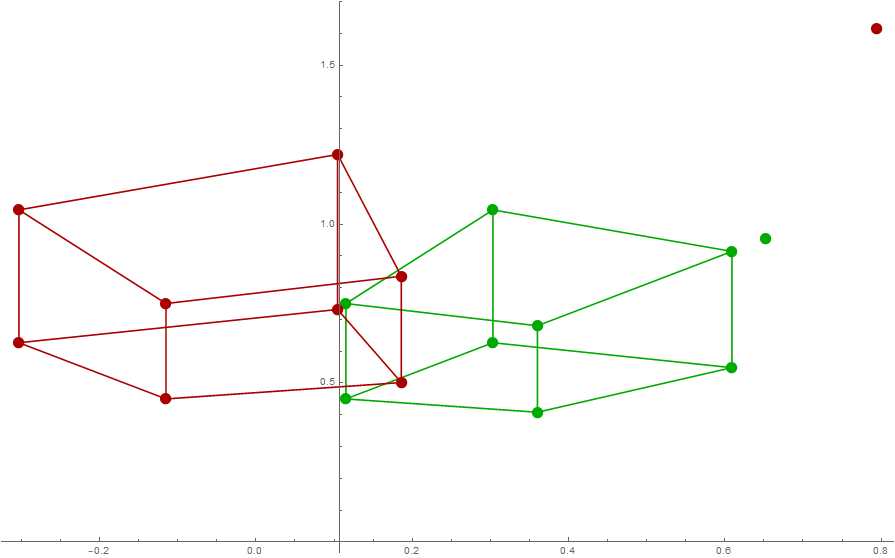
\includegraphics[width=.8\linewidth]{images/Rectification_one_same_Solutions.png}
	\captionof{figure}{Aufnahmen zweier Kameras mit den selben Auflösungen, Kamera eins(Grün) und Kamera(rot) zwei gelten jeweils \ensuremath{\zeta =1}} 
\end{minipage}\\ 

\begin{minipage}{\linewidth}
	\centering
	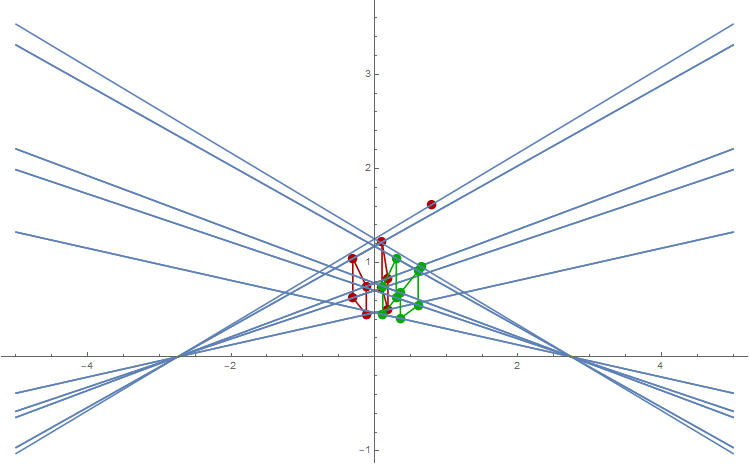
\includegraphics[width=.8\linewidth]{images/Rectification_two_same_Solutions.png}
	\captionof{figure}{Epipole für Kamera eins und Kamera zwei vor der Rektifizierung } 
\end{minipage}\\


Werden nun die Matritzen $H_p$ und $H_p'$ auf die jeweiligen Punkte der Bilder, $p_i$ für Bild eins und $p_j$ für Bild zwei, angewandt, so kann man eine erste Veränderung beobachten. Abbildung 4.9 zeigt beide Quader aus Abbildung 4.7 nachdem die jeweiligen Bildpunkte mit den projektiven Matrizen multipliziert wurden. Der Epipol in Bild eins bleibt natürlich wie zuvor im unendlichen, jedoch kann man erkennen, dass der rote Quader aus Bild zwei sich verändert hat. Sein Epipol wurde ins Unendliche transformiert und parallele Linien sind nun auch auf dem Bild parallel. Das die Epipolarlinien bereits horizontal parallel zur x-Achse verlaufen ist Zufall und ist nach der Anwendung der projektiven Matrizen auch noch nicht verlangt. Das Anpassen der Epipolarlinien, dazu gehört sie zunächst von beiden Bilder aus parallel zur x-Achse verlaufen zu lassen und dann noch sie so zueinander anzupassen, dass sie zu Scanlinien über beide Bilder verlaufen, verlgeiche Abbildung 4.12, folgt im nächsten Schritt. \\


\begin{minipage}{\linewidth}
	\centering
	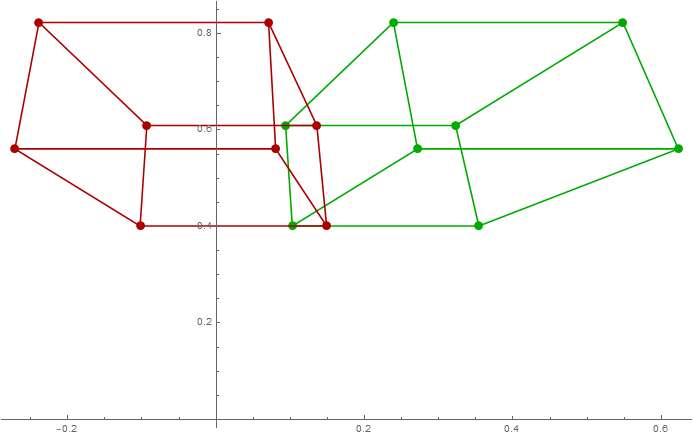
\includegraphics[width=1.\linewidth]{images/Rectification_Hp_same_Solutions.png}
	\captionof{figure}{Abbildung beider Bilder nach anwenden der Matrizen $H_p$ und $H_p'$. Die Epipole beider Bilder sind nun im unendlichen. Das die enstehenden parallelen Epipolarlinien auch hier schon horizontal ausgerichtet sind ist Zufall. Die Epipolarlinien sind immer parallel nach dieser Transformation aber die Richtung ist nicht immer automatisch bereits i = [1,0,0].} 
\end{minipage}\\ \\

\section{Ähnlichkeitstransformation}

Nachdem die Epipole ins Unendliche verschoben wurden, müssen diese nun so rotiert und verschoben werden, dass die Epipolarlinien als Richtung $i = \begin{bmatrix}1&0&0\end{bmatrix}$ haben und die Epipolarlinien beider Bilder zu einheitlichen Scanlinien werden. Für die Ähnlichkeitstransformation wird davon ausgegangen, dass $w$ und $w'$ bereits bekannt sind.$H_r$ und $H_r'$ wurden bereits aus der Zerlegung von $H_a$ und $H_a'$ gewonnen.

\begin{gather}
		H_r = 
	\begin{bmatrix}
	v_b-v_cw_b&	v_a-v_cw_a&0\\
	v_a-v_cw_a&v_b-v_cw_b&v_c\\
	0&0&1
	\end{bmatrix}\\
		H_r' = 
	\begin{bmatrix}
	v_b'-v_c'w_b'&	v_a'-v_c'w_a'&0\\
	v_a'-v_c'w_a'&v_b'-v_c'w_b'&v_c'\\
	0&0&1
	\end{bmatrix}\\
\end{gather}

$w$ und $w'$ sind bereits bekannt, Mit Hilfe von $F$, können $v_a$ und $v_b$ ersetzt werden. Dazu kann die letzte Zeile von F nach $v_a, v_b$ und $v_c$ aufgelöst werden. Für $v_a', v_b'$ und $v_c'$ wird die letzte Spalte von F verwendet. So können folgende Gleichungen für $v_a, v_a',v_b, v_b', v_c$ und $v_c'$ gewonnen werden. 

\begin{gather}
	F = H'^T[i]_xH\\
	F=
	\begin{bmatrix}
	v_aw_a' - v_a'w_a&v_bw_a' - v_a'w_b&v_cw_a' - v_a'\\
	v_aw_b' - v_b'w_a&v_bw_b' - v_b'w_b&v_cw_b' - v_b'\\
	v_a - v_c'w_a&v_b - v_c'w_b&v_c-v_c'
	\end{bmatrix}\\
	v_a = F_{31}+v_c'w_a\\
	v_b = F_{32}+v_c'w_b\\
	v_c = F_{33}+v_c'\\
	v_a' = v_cw_a'-F_{13}\\
	v_b' = v_cw_b'-F_{23}\\
	v_c' = v_c -F_{33}
\end{gather}

Eingesetzt in die jeweiligen Matrizen $H_r$ und $H_r'$, entstehen die folgenden Matrizen in Gleichungen 4.114 und 4.115, welche nur noch die unbekannte $v_c'$ beinhalten. Die gemeinsame Variable $v_c'$ zeigt die geometrische Verbindung beider Bilder in ihrer Verschiebung entlang ihrer v-Richtung. Es wird also ein Offset von $F_33$ benötigt, um die Epipolarlinien horizontal zu Scanlinien auszurichten. \textcolor{red}{Den Wert für $v_c$ wird so ermittelt, dass das Minimum einer v-Koordinaten eines Pixel als minimum den Wert null besitzt }

\begin{gather}
	H_r = \begin{bmatrix}
	F_{32}-w_bF_{33}&w_aF_{33}-F_{31}&0\\
	F_{31}-w_aF_{33}&F_{32}-w_bF_{33}&F_{33}+v_c'\\
	0&0&1
	\end{bmatrix}\\
	H_r'=
	\begin{bmatrix}
	w_b'F_{33}-F_{23}&F_{13}-w_a'F_{33}&0\\
	w_a'F_{33}-F_{13}&w_b'F_{33}-F_{23}&v_c'\\
	0&0&1
	\end{bmatrix}
\end{gather}\\

Das Ergebnis der Bildpunkte $p_i$ und $p_j$ multipliziert mit den Matrizen $H_rH_p$ und $H_r'H_p'$ mit ist in Abbildung 4.10 zu sehen. Als letztes folgt noch die Scherungstransformation $H_s$ und $H_s'$ für die horizontale Entzerrung beider Bilder.\\ 

\begin{minipage}{\linewidth}
	\centering
	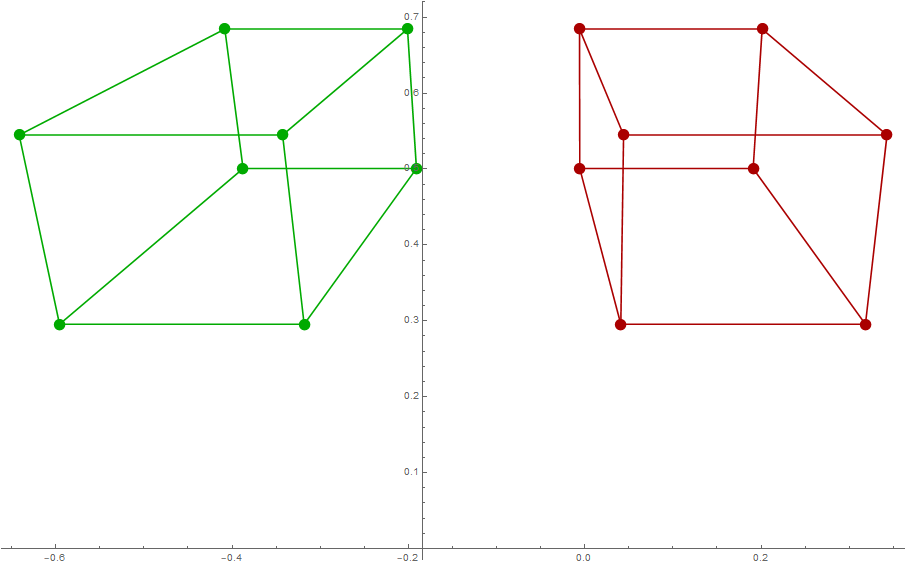
\includegraphics[width=1.\linewidth]{images/Rectification_HrHp_same_Solutions.png}
	\captionof{figure}{Abbildung beider Bilder nach anwenden der Matrizen $H_r \cdot H_p$ und $H_r' \cdot H_p'$. Die Epipolarlinien sind nun horizontal zueinander ausgerichtet} 
\end{minipage}\\ \\

\section{Scherungstransformation}

Die letzte Transformation, welche an den Bilder durchgeführt werden soll, ist die sogenannten Scherungstransformation. Sie soll vor allem dazu dienen, die horizontale Verzerrung der Bilder zueinander nochmal weiter zu minimieren. Die Matrizen $H_s$ und $H'_r$ wirken sich hauptsächlich auf die $u$ und $u'$ Komponenten aus. 

\begin{gather}
	H_s =\begin{bmatrix}
	u_a&u_b&0\\
	0&1&0\\
	0&0&1
	\end{bmatrix}\\
		H'_s =\begin{bmatrix}
	u'_a&u'_b&0\\
	0&1&0\\
	0&0&1
	\end{bmatrix}
\end{gather}

Um die richtigen Werte für $a, a', b$ und $b'$ zu bekommen, werden zunächst Punkte an den jeweiligen gegenüberliegenden Kanten der Bilder definiert. Da die Bilder des Quaders nicht aus tausenden von Pixeln bestehen, wie ein reales Bild, sondern nur über dessen Eckpunkte bestimmt ist, wird eine Bildbreite $w$ und $w'$ und eine Bildhöhe $h$ und $h'$ definiert. Die Höhen und Breiten der Bilder rahmen die abgebildeten Quader ein, somit wurde quasi eine Bildgröße für beide Bilder definiert. Nun können die Punkte an den Kantenhalbierenden $a = [\frac{w-1}{2} \; 0 \; 1]^T, b = [w-1 \; \frac{h-1}{2}\; 1]^T, c = [\frac{w-1}{2} \; h-1 \; 1]^T, d = [0 \; \frac{h-1}{2} \; 1]^T$ gebildet werden. Der Gedanke, der damit verfolgt wird ist, dass die Punkte der jeweiligen gegenüberliegenden Kanten mit einander verbunden werden können und dann so ausgerichtet werden sollen, dass sie sich wieder direkt gegenüber liegen. Schematisch wird as in Abbildung ???? aufgezeigt.

\begin{minipage}{\linewidth}
	\centering
	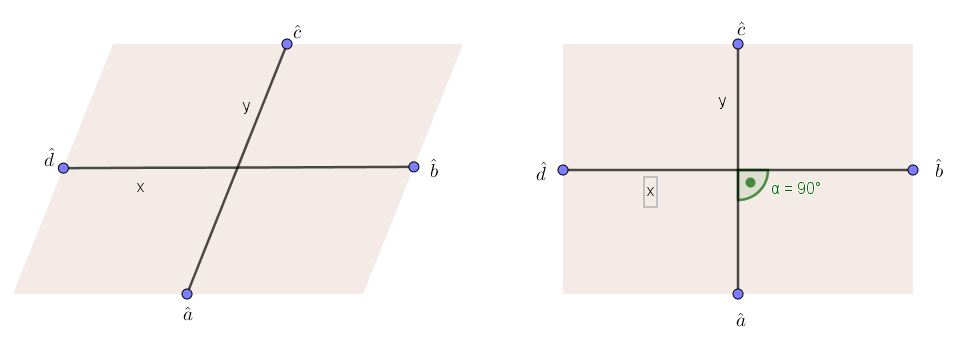
\includegraphics[width=.8\linewidth]{images/Scherungstransformation.png}
	\captionof{figure}{Die Abbildung verdeutlicht noch mal Schematisch, wie sich die Punkte ausrichten sollen. Bild a) zeigt die durch die Rektifizierung verschobenen Bildkantenmitten. Bild b= zeigt, wie sich die Bildkantenmitten durch die Scherungstransformation wieder ausrichten sollen.} 
\end{minipage}\\ \\

Die Punkte $a,b,c,d$ und auch $a',b',c',d'$ geben die Bildbreiten der noch unberührten Bilder an. Nach der Rektifizierung sind die Bilder so verzerrt, dass die Kanten mitten sich meistens nicht mehr direkt gegenüber von einander befinden. Die Punkte $a,b,c,d$ und $a',b',c',d'$ werden mit den Matrizen $H_p, H'_p, H_r$ und $H'_r$ verrechnet, so dass man die genaue neue Position der Kanten Mitten nach der Rektifizierung hat. 

\begin{gather*}
	\hat{a} = H_r\cdot H_p \cdot a\\
	\hat{b} = H_r\cdot H_p \cdot b\\
	\hat{c} = H_r\cdot H_p \cdot c\\
	\hat{d} = H_r\cdot H_p \cdot d\\
	\hat{a'} = H'_r\cdot H'_p \cdot a'\\
	\hat{b'} = H'_r\cdot H'_p \cdot b'\\
	\hat{c'} = H'_r\cdot H'_p \cdot c'\\
	\hat{d'} = H'_r\cdot H'_p \cdot d'\\
\end{gather*}

Um aus $\hat{a},\hat{b},\hat{c},\hat{d}$ und auch $\hat{a}',\hat{b}',\hat{c}',\hat{d}'$ wieder Punkte der affinen Ebene zu machen werden sie jeweils durch ihre dritte Komponenten geteilt, so das $\hat{a}_w,\hat{b}_w,\hat{c}_w,\hat{d}_w$ und $\hat{a}'_w,\hat{b}'_w,\hat{c}'_w,\hat{d}'_w$ jeweils den Wert eins besitzen. Danach können die Vektoren $\vec{x}$ und $\vec{y}$ aus den Differenzen der sich ursprünglich gegenüberliegenden Punkte gebildet werden.

\begin{gather}
	x = \hat{b}-\hat{d}\\
	y = \hat{c}-\hat{a}\\
	x' = \hat{b}'-\hat{d}'\\
	y' = \hat{c}'-\hat{a}'
\end{gather}

$x$ und $y$ sind Vektoren der euklidischen Bildebene. Die Rechwinkligkeit beider wird also erhalten, wenn gilt:

\begin{gather}
	(H_sx)^T(H_sy)= 0 \\
	(H'_sx')^T(H'_sy')= 0 
\end{gather}

Die Seitenverhältnisse der Bilder werden beibehalten, wenn gilt:

\begin{gather}
	\frac{(H_sx)^T(H_sx)}{(H_sy)^T(H_sy)} = \frac{w^2}{h^2}\\
	\frac{(H'_sx')^T(H'_sx')}{(H'_sy')^T(H'_sy')} = \frac{w'^2}{h'^2}	
\end{gather}

Für $u_a, u'_a, u_b$ und $u'_b$ jeweils Gleichungen auf Basis der jeweiligen Bild Höhen und Breiten $w,w',h,h'$ und $x,x',y$ und $y'$ und unter einhaltung der Aussagen der Gleichungen 5.118 bis 5.121, aufgestellt werden\cite{ZZ,ACM}. 

\begin{gather}
	u_a = \frac{h^2x_v^2+w^2+y_v^2}{hw(x_vy_u-x_uy_v)}\\
	u_b = \frac{h^2x_ux_v+w^2y_uy_v}{hw(x_uy_v-x_vy_u)}
\end{gather}

Selbe Gleichungen werden auch für $u'_a$ und $u'_b$ aufgestellt. Das Ergebnis der Scherungstransformation ist in Abbildung 5.17 dargestellt. \textcolor{red}{ Wie zu sehen ist, ist die Minimierung noch nicht zu hindert prozent perfekt, hierfür müsste man noch ein paar mehr Interationsschritte bei finden von $z$ einfügen.}(ICH WEIß GANZ EHRLICH NICHT WORAN ES LIEGT...)


\begin{minipage}{\linewidth}
	\centering
	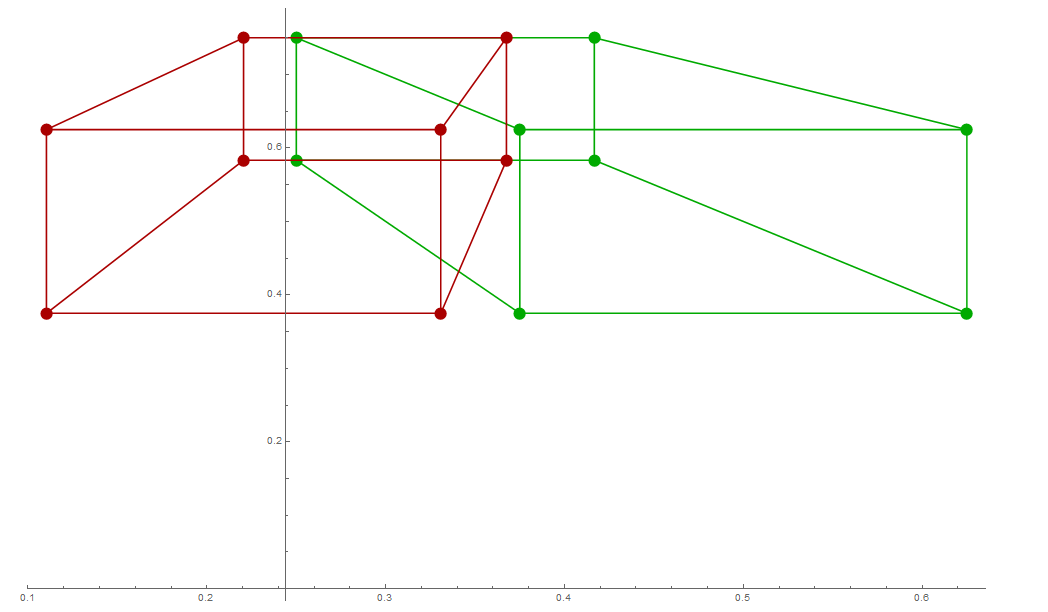
\includegraphics[width=1.\linewidth]{images/Rectification_HsHrHp_same_Solutions.png}
	\captionof{figure}{Abbildung beider Bilder nach anwenden der Matrizen $H_s \cdot H_r \cdot H_p$ und $H_s' \cdot H_r' \cdot H_p'$. Die horizontale Verzerrung wurde reduziert.} 
\end{minipage}\\ \\

\begin{minipage}{\linewidth}
	\centering
	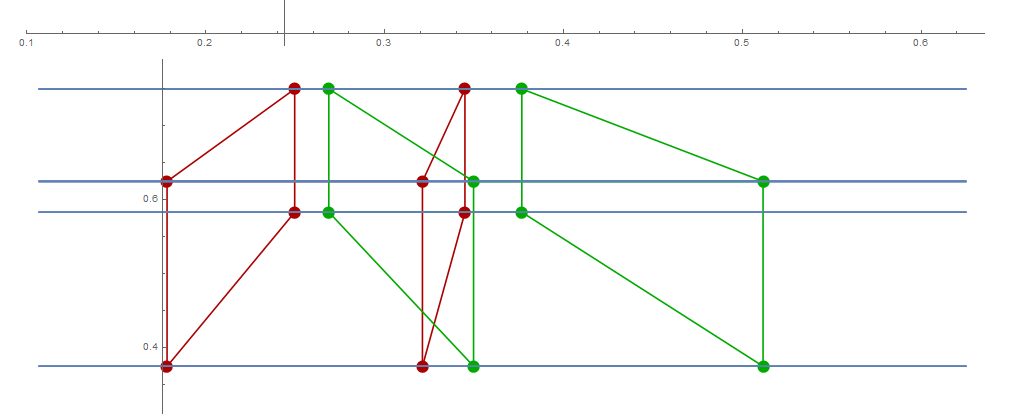
\includegraphics[width=1.\linewidth]{images/Rectification_four_same_Solutions.png}
	\captionof{figure}{In dieser Abbildung wurden die Epipolarlinien noch in den Grafikplot mit eingebaut} 
\end{minipage}\\ \\

%\begin{minipage}{\linewidth}
%	\centering
%	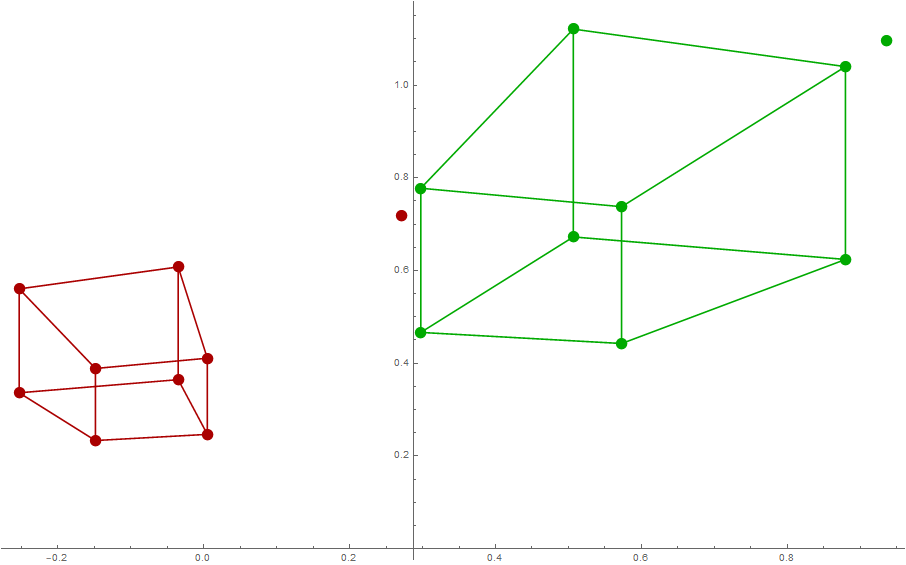
\includegraphics[width=1.\linewidth]{images/Rectification_one_different_Solutions.png}
%	\captionof{figure}{Aufnahmen zweier Kameras mit unterschiedlichen auflösungen, Kamera eins(Grün) besitzt für \ensuremath{\zeta} den Wert 1 und für Kamera zwei(rot) gilt jeweils \ensuremath{\zeta_x = 1.2} und \ensuremath{\zeta_y = 3.1}} 
%\end{minipage}\\ \\
%
%(Normalerweise in realbildern wird das bild bei unterschiedlicher Auflösung nicht verzerrt sondern nur "Vergrößert" oder zurecht "geschnitten". Dadruch dass beide Quader in einem Koordinatensystem verbaut wurden sieht das so aus)
%
%
%\begin{minipage}{\linewidth}
%	\centering
%	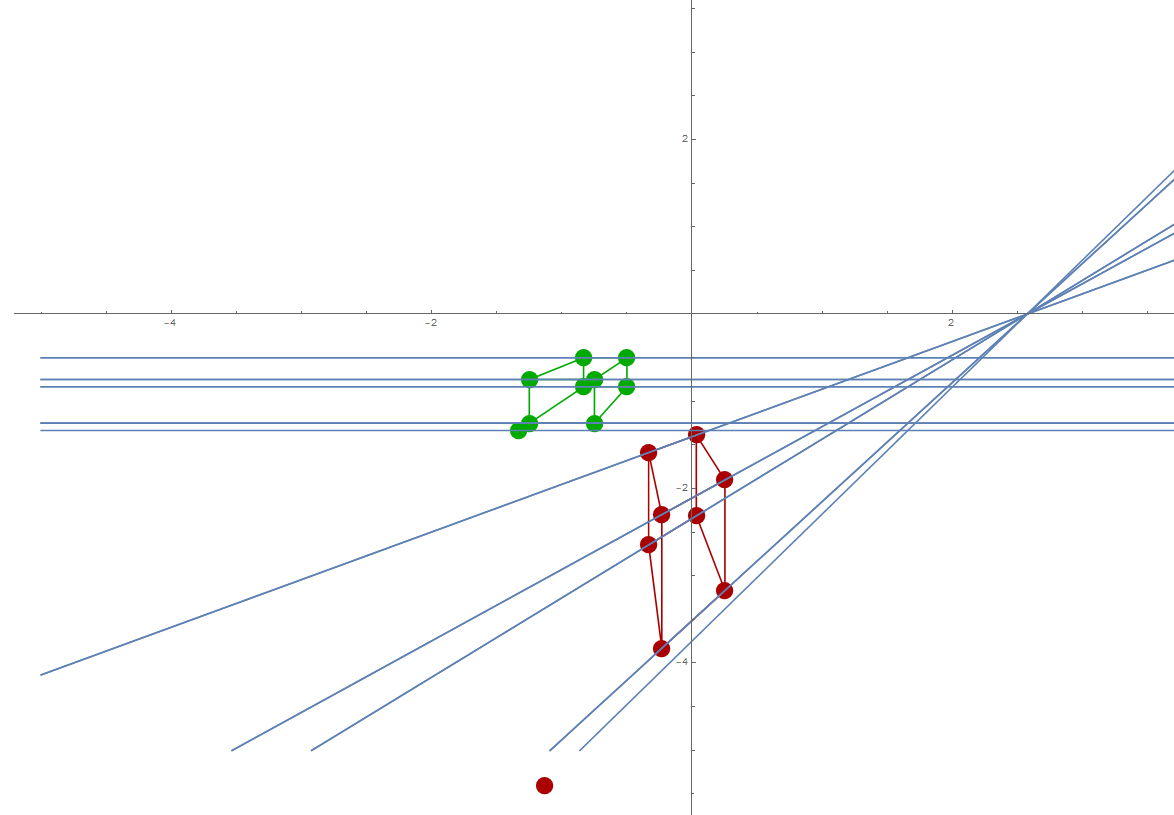
\includegraphics[width=1.\linewidth]{images/Rectification_two_different_Solutions.png}
%	\captionof{figure}{Epipole für Kamera eins und Kamera zwei vor der Rektifizierung } 
%\end{minipage}\\ \\
%
%
%\begin{minipage}{\linewidth}
%	\centering
%	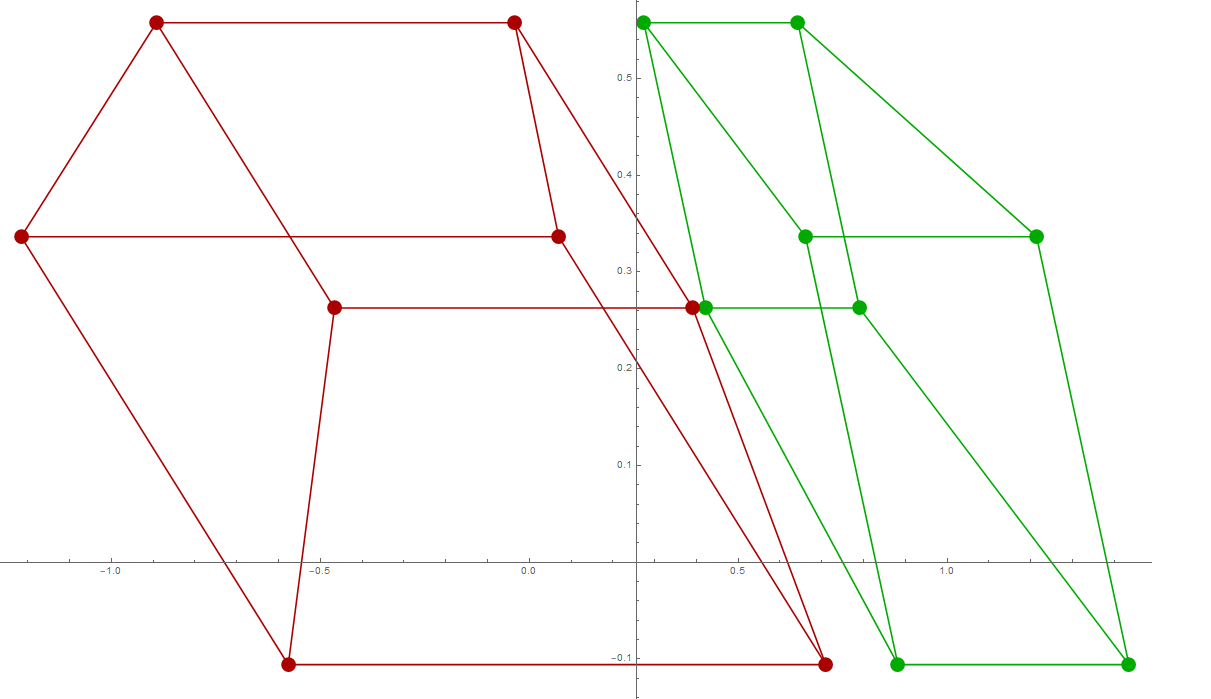
\includegraphics[width=1.\linewidth]{images/Rectification_three_different_Solutions.png}
%	\captionof{figure}{Nach dem die drei Homographien auf die Punkte angewandt sind die Eckpunkte des Quaders auf beiden Bilder auf den selben corresüondierenden Epipolarlinien} 
%\end{minipage}\\ \\
%
%
%\begin{minipage}{\linewidth}
%	\centering
%	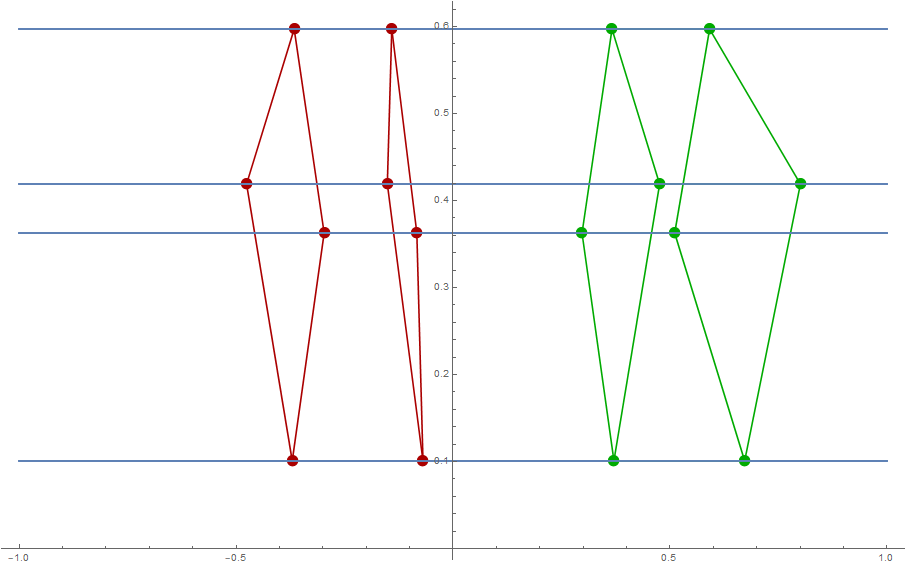
\includegraphics[width=1.\linewidth]{images/Rectification_four_different_Solutions.png}
%	\captionof{figure}{In dieser Abbildung wurden die Epipolarlinien noch in den Grafikplot mit eingebaut} 
%\end{minipage}\\ \\
